\documentclass[12pt]{article}

\usepackage[margin=1in]{geometry}
\usepackage{amsmath,amsthm,amssymb}
\usepackage{mathtools}
\usepackage{mathrsfs}
\usepackage{enumitem}
\usepackage{physics}

\usepackage{tikz}
\usetikzlibrary{calc,decorations.markings,patterns}

\newcommand{\magsq}[1]{\big|#1\big|^2}
\newcommand{\avg}[1]{\left<#1\right>}
\newcommand{\fullint}{\int_{-\infty}^\infty}
\newcommand{\fullintd}[1]{\fullint\dd#1\:}
\newcommand{\cint}[2]{\int_{#1}^{#2}}
\newcommand{\cintd}[3]{\cint{#1}{#2}\dd#3\:}

\begin{document}

\title{Homework 1}
\author{Sean Ericson \\ Phys 611}
\maketitle

\section*{Problem 1}
\begin{enumerate}[label=(\alph*)]
    \item To start with, we need to parameterize a path along the surface of a sphere (along with it's derivative w.r.t. the parameter $\phi$):
    \[ \vec{r}(\phi) = \mqty(r\sin\theta\cos\phi \\ r\sin\theta\sin\phi \\ r\cos\theta) \]
    \[ \dot{\vec{r}} = r\mqty(\cos\theta\cos\phi\dot{\theta} - \sin\theta\sin\phi \\ \cos\theta\sin\phi\dot{\theta} + \sin\theta\cos\phi \\ -\sin\theta\dot{\theta}) \]
    The arc length is then given by
    \[ S = \cintd{\phi_0}{\phi_1}{\phi} |\dot{\vec{r}}| \]
    Now,
    \begin{align*}
        \magsq{\dot{\vec{r}}} &= \cos^2\theta\cos^2\phi\dot{\theta}^2 - 2\cos\theta\sin\theta\cos\phi\sin\phi\dot{\theta}  \\ 
        &+ \sin^2\theta\sin^2\phi + \cos^2\theta\sin^2\phi\dot{\theta}^2 + 2\cos\theta\sin\theta\cos\phi\sin\phi\dot{\theta} + \sin^2\theta\cos^2\phi + \sin^2\theta\dot{\theta}^2 \\
        & = \cos^2\theta\cos^2\phi\dot{\theta}^2 + \cos^2\theta\sin^2\phi\dot{\theta}^2 + \sin^2\theta\sin^2\phi + \sin^2\theta\cos^2\phi + \sin^2\theta\dot{\theta}^2 \\
        &= \cos^2\theta\dot{\theta}^2 + \sin^2\theta + \sin^2\theta\dot{\theta}^2 \\
        &= \dot{\theta}^2 + \sin^2\theta
    \end{align*}
    so the arc length is then
    \[ \boxed{S = r\cintd{\phi_0}{\phi_1}{\phi}\sqrt{  \dot{\theta}^2 + \sin^2\theta}} \]
    where $\theta$ and $\dot{\theta}$ are both functions of $\phi$.
    \item Let's take some derivatives!
    \begin{align*}
        \pdv{\mathscr{L}}{\theta} &= \frac{\sin\theta\cos\theta}{\sqrt{\dot{\theta}^2 + \sin^2\theta}} \\
        \pdv{\mathscr{L}}{\dot{\theta}} &= \frac{\dot{\theta}}{\sqrt{\dot{\theta}^2 + \sin^2\theta}} \\
        \dv{t}\pdv{\mathscr{L}}{\dot{\theta}} &= \frac{\ddot{\theta}}{\sqrt{\dot{\theta}^2 + \sin^2\theta}} - \frac{\dot{\theta}^2\left(\ddot{\theta} + \sin\theta\cos\theta\right)}{\left(\dot{\theta}^2 + \sin^2\theta\right)^{3/2}} 
    \end{align*}
    The Euler-Lagrange equation then gives
    \[ \frac{\sin\theta\cos\theta}{\sqrt{\dot{\theta}^2 + \sin^2\theta}} = \frac{\ddot{\theta}}{\sqrt{\dot{\theta}^2 + \sin^2\theta}} - \frac{\dot{\theta}^2\left(\ddot{\theta} + \sin\theta\cos\theta\right)}{\left(\dot{\theta}^2 + \sin^2\theta\right)^{3/2}} \]
    which simplifies (somewhat) to
    \[ \boxed{ \sin\theta\cos\theta = \ddot{\theta} - \frac{\dot{\theta}^2(\ddot{\theta} + \sin\theta\cos\theta)}{\left(\dot{\theta}^2 + \sin^2\theta\right)^3}} \]
    \item c
\end{enumerate}

\section*{Problem 2}
\begin{enumerate}[label=(\alph*)]
    \item Extending the derivation from class, now for $\mathscr{L}(y, \dot{y}, \ddot{y})$, 
    \[ \delta\mathscr{L} = \left(\pdv{\mathscr{L}}{x}\right)\delta x + \left(\pdv{\mathscr{L}}{\dot{x}}\right)\delta\dot{x} + \left(\pdv{\mathscr{L}}{\ddot{x}}\right)\delta\ddot{x} \]
    Integrating by parts once on the second term and twice on the third term yields
    \[ \delta S = \cintd{x_0}{x_1}{x} \left(\pdv{\mathscr{L}}{x} - \dv{x}\pdv{\mathscr{L}}{\dot{x}} + \dv[2]{x}\pdv{\mathscr{L}}{\ddot{x}}\right)\delta x \]
    Now we can use the stationary action principle to derive the modified Euler-Lagrange equation
    \[ \delta S = 0 \implies \boxed{\pdv{\mathscr{L}}{y} - \dv{x}\pdv{\mathscr{L}}{\dot{y}} + \dv[2]{y}\pdv{\mathscr{L}}{\ddot{x}} = 0} \]
    
    \item Now to apply the modified EL equation. The Lagrangian is given by
    \[ \mathscr{L}(y, \dot{y}, \ddot{y}) = \ddot{y}^2 \]
    Now some derivatives!
    \[ \pdv{\mathscr{L}}{y} = 0; \quad \pdv{\mathscr{L}}{\dot{y}} = 0; \quad \pdv{\mathscr{L}}{\ddot{y}} = 2\ddot{y} \]
    \[ \dv[2]{x}\pdv{\mathscr{L}}{\ddot{y}} = 2\ddddot{y} \]
    The Euler-Lagrange equation then gives
    \[ \ddddot{y} = 0 \]

    \item The general solution to the above equation is
    \[ y(x) = ax^3 + bx^2 + cx + d \]
    Applying the boundary conditions $y(0) = 0$ and $y'(0) = 0$ gives
    \[ c = d = 0 \]
    Further, applying the boundary conditions $y(L) = h$ and $y'(L) = m$ gives
    \[  \]
\end{enumerate}


\section*{Problem 3}
\begin{center}
    \scalebox{5}{
        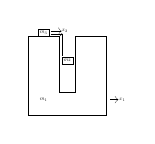
\begin{tikzpicture}[line width=0.1pt]
            \draw (0,0) -- (1,0) -- (1,1) -- (0.6,1) -- (0.6, 0.3) -- (0.4, 0.3) -- (0.4, 1) -- (0, 1) -- cycle;
            % \draw (0.2, 1) -- (0.3, 1) -- (0.3, 1.1) -- (0.2, 1.1) -- cycle;
            \filldraw (0.43,1.03) circle (0.25pt);
            \draw (0.4,1) -- (0.43,1.03);
            \node at (0.2,1.05) [rectangle,draw,scale=0.2] {$m_3$};
            \node at (0.5,.7) [rectangle,draw,scale=0.2] {$m_2$};
            \node at (0.2, 0.2) [scale=0.2] {$m_1$};
            \draw (0.29,1.03) -- (0.43,1.03) -- (0.43,0.75);
            \draw [-to](.3,1.07) -- (.43, 1.07);
            \node at (0.47, 1.07) [scale=0.2] {$x_2$};
            \draw [-to](1.05, 0.2) -- (1.15, 0.2);
            \node at (1.2,0.2)[scale=0.2]{$x_1$};
        \end{tikzpicture}
    }
\end{center}

\begin{enumerate}[label=(\alph*)]
    \item Taking $x_1$ and $x_2$ as the independent variables (with $x_1$ measured relative to the ground and $x_2$ relative to $m_1$), the kinetic energy of each mass is given by
    \begin{align*}
        T_1 &= \frac{1}{2}m_1\dot{x}_1^2 \\
        T_2 &= \frac{1}{2}m_2(\dot{x}_1^2 + \dot{x}_2^2) \\
        T_3 &= \frac{1}{2}m_3(\dot{x}_1 + \dot{x}_2)^2
    \end{align*}
    The only relevant potential energy is that of $m_2$:
    \[ U = -m_2gx_2 \]
    This gives a Lagrangian of
    \[ \boxed{\mathscr{L} = \frac{1}{2}m_1\dot{x}_1^2 + \frac{1}{2}m_2(\dot{x}_1^2 + \dot{x}_2^2) + \frac{1}{2}m_3(\dot{x}_1 + \dot{x}_2)^2 + m_2gx_2} \]
    \item Let's take some derivatives!
    \begin{align*}
        \pdv{\mathscr{L}}{x_1} &= 0 \\
        \pdv{\mathscr{L}}{\dot{x}_1} &= m_1\dot{x}_1 + m_2\dot{x}_1 + m_3(\dot{x}_1 + \dot{x}_2) \\
        &= (m_1+m_2+m_3)\dot{x}_1 + m_3\dot{x}_2 \\
        \dv{t}\pdv{\mathscr{L}}{\dot{x}_1} &= (m_1+m_2+m_3)\ddot{x}_1 + m_3\ddot{x}_2 \\
        \\
        \pdv{\mathscr{L}}{x_2} &= m_2g \\
        \pdv{\mathscr{L}}{\dot{x}_2} &= m_2\dot{x}_2 + m_3(\dot{x}_1 + \dot{x}_2)  \\
        &= (m_2+m_3)\dot{x}_2 + m_3\dot{x}_1 \\
        \dv{t}\pdv{\mathscr{L}}{\dot{x}_1} &= (m_2+m_3)\ddot{x}_2 + m_3\ddot{x}_1 \\
    \end{align*}
    Applying the Euler-Lagrange equation gives the (coupled) equations of motion
    \begin{alignat*}{4}
        (m_1+m_2+m_3)\ddot{x}_1+&&\quad m_3&&\ddot{x}_2 =&& 0 \\
        m_3\ddot{x}_1+&&\quad (m_2+m_3)&&\ddot{x}_2 =&& m_2g
    \end{alignat*}
    which can equivalently be written as
    \[ \mqty(m_1+m_2+m_3 & m_3 \\ m_3 & m_2+m_3)\mqty(\ddot{x}_1 \\ \ddot{x}_2) = \mqty(0 \\ m_2g) \]
    Inverting the above equation to solve for $\ddot{x}_1$ and $\ddot{x}_2$ yields
    \begin{align*}
        \mqty(\ddot{x}_1 \\ \ddot{x}_2) &= \frac{1}{(m_1+m_2+m_3)(m_2+m_3) - m_3^2}\mqty(m_2+m_3 & -m_3 \\ -m_3 & m_1+m_2+m_3)\mqty(0 \\ m_2g) \\
        &= \frac{1}{(m_1+m_2+m_3)(m_2+m_3) - m_3^2}\mqty(-m_2m_3 \\ (m_1+m_2+m_3)m_2g)
    \end{align*}
    Reading off the first component gives the acceleration of $m_1$
    \[ \boxed{\ddot{x}_1 = \frac{-m_2m_3g}{(m_1+m_2+m_3)(m_2+m_3) - m_3^2}} \]
\end{enumerate}



\section*{Problem 4}
\begin{enumerate}[label=(\alph*)]
    \item Since there's no potential energy, the Lagrangian is just the kinetic energy:
    \begin{align*}
        \mathscr{L} &= T \\
        &= \frac{1}{2}m(r^2\dot{\theta}^2 + v_0^2) \\
        &= \frac{1}{2}m(v_0^2t^2\dot{\theta}^2 + v_0^2) \\
        &= \boxed{\frac{1}{2}mv_0^2(\dot{\theta}^2t^2 + 1)}
    \end{align*}
    \item Let's take some derivatives!
    \begin{align*}
        \pdv{\mathscr{L}}{\theta} &= 0 \\
        \pdv{\mathscr{L}}{\dot{\theta}} &= mv_0^2\dot{\theta}t^2 \\
        \dv{t}\pdv{\mathscr{L}}{\dot{\theta}} &= mv_0^2(\ddot{\theta}t^2 + 2\dot{\theta}t)
    \end{align*}
    Applying the Euler-Lagrange equation yields
    \[ mv_0^2(\ddot{\theta}t^2 + 2\dot{\theta}t) = 0 \implies \boxed{t\ddot{\theta} + 2\dot{\theta} = 0}\]
    \item The general solution for the above differential equation is
    \[ \theta(t) = \frac{a}{t} + b \]
    Plugging in the given initial conditions gives
    \begin{align*}
        \frac{a}{t_0} + b &= 0 \\
        -\frac{a}{t_0^2} &= \omega_0
    \end{align*}
    Solving for the constants of integration gives
    \begin{align*}
        a &= -\frac{\omega_0}{t_0^2} \\
        b &= -t_0\omega_0
    \end{align*}
    The exact solution is then
    \[ \boxed{\theta(t) = -\frac{t_0^2\omega_0}{t} - t_0\omega_0 = -t_0\omega_0\left(\frac{t_0}{t} + 1\right)} \]
\end{enumerate}


\section*{Problem 5}

\begin{center}
    \scalebox{.75}{
        \begin{tikzpicture}
            \draw (5,5) circle (5);
            \draw [dashed] (5,5) -- (10,5);
            \draw [dashed] (10,5) -- (10,-4);
            \node at (10,0) [right] {$l$};
            \filldraw [pattern=north west lines] (10,-4) circle (0.1);
            \node at (7.5,5.3) {$R$};
            \draw [->] (5,5) -- (8.5,1.5);
            \node at (8.5,2) {$\vec{P}$};
            \begin{scope}
                \path[clip] (5,5) -- (10,5) -- (8.5,1.5) -- cycle;
                \node[circle,draw,minimum size=45pt] at (5,5) (circ) {};
            \end{scope}
            \node at (6.2,4.5) {$\theta$};
            \draw (8.55,1.45) -- (4.5,-2);
            \node at (6.6,-0.55) {$l'$};
            \filldraw (4.5,-2) circle (0.1);
            \node at (4.5,-2) [right] {$m$};
            \draw [->] (5,5) -- (4.5,-1.9);
            \node at (4,-1.5) {$\vec{r}$};
            \draw [->] (5,8) -- (7,8);
            \node at (6,8) [above] {$x$};
            \draw [->] (5,8) -- (5,6);
            \node at (5,7) [left] {$y$};
        \end{tikzpicture}
    }
\end{center}
\begin{enumerate}[label=(\alph*)]
    \item First, some needed quantities/vectors
    \[ l' = l - R\theta \]
    \[ \vec{r} - \vec{p} = \mqty(-l'\sin\theta \\ l'\cos\theta) \]
    \[ \implies \vec{r} = \mqty(-l'\sin\theta + R\cos\theta \\ l'\cos\theta + R\sin\theta) = \mqty(-(l-R\theta)\sin\theta + R\cos\theta \\ (l-R\theta)\cos\theta + R\sin\theta) \]
    The kinetic and potential energies are given by
    \begin{align*}
        T &= \frac{1}{2}m\magsq{\dot{\vec{r}}} \\
        &= \frac{1}{2}m\mqty|R\sin\theta\dot{\theta} - (l-R\theta)\cos\theta\dot{\theta} - R\sin\theta\dot{\theta} \\ -R\cos\theta\dot{\theta} - (l-R\theta)\sin\theta\dot{\theta} + R\cos\theta\dot{\theta}|^2 \\
        &= \frac{1}{2}m\mqty|(R\theta-l)\cos\theta\dot{\theta} \\ (R\theta - l)\sin\theta\dot{\theta}|^2 \\
        &= \frac{1}{2}m\dot{\theta}^2(R\theta - l)^2 \\
        \\
        V &= -mg(\vec{r}\cdot\hat{y}) \\
        &= -mg\left((l-R\theta)\cos\theta + R\sin\theta\right)
    \end{align*}
    Combining these, we get the Lagrangian
    \[ \boxed{\mathscr{L} = \frac{1}{2}m\dot{\theta}^2 + mg(l-R\theta)\cos\theta + mgR\sin\theta} \]
    
    \item Let's take some derivatives!
    \begin{align*}
        \pdv{\mathscr{L}}{\theta} &= m\dot{\theta}^2(R\theta - l) - mgR\cos\theta - mg(l-R\theta)\sin\theta + mgR\cos\theta \\
        &= m\dot{\theta}^2(R\theta - l) - mg(l-R\theta)\sin\theta \\
        \\
        \pdv{\mathscr{L}}{\dot{\theta}} &= m\dot{\theta}(R\theta - l)^2 \\
        \dv{t}\pdv{\mathscr{L}}{\dot{\theta}} &= m\ddot{\theta}(R\theta - l)^2 + 2m\dot{\theta}(R\theta - l)
    \end{align*}
    The Euler-Lagrange equation is now
    \[ m\dot{\theta}(R\theta -l)^2 = m\ddot{\theta}(R\theta - l)^2 + 2m\dot{\theta}(R\theta - l) \]

    \item c
\end{enumerate}

\end{document}